\begin{frame}{Plan}
  \setbeamertemplate{section in toc}[sections numbered]
  \tableofcontents[hideallsubsections]
\end{frame}

\section{\'Etat de l'art de la production automatique de mots-clés}

\begin{frame}<1-2>[label=productionauto]{Méthodes de production automatique de mots-clés}
    \begin{figure}
    \centering
    \begin{tikzpicture}
    
    \pic[local bounding box=doc] at (-4,0) {doc={scale 1.5}};
    \node[below=.5cm of doc] {Document};

    \pic[local bounding box=ch doc] at (-1,2) {doc={scale .75}};
    \pic[local bounding box=ch cand, right=.5 of ch doc] {dockw={scale .75}};
    \pic[local bounding box=ch weigh, right=.375 of ch cand] {weighted={scale .375}};
    \pic[local bounding box=ch kws, right=.375 of ch weigh] {kws={scale .375}};
    \node[text width=3cm, align=center, below=.5cm of ch doc] (ch label) at ($(ch doc)!.5!(ch kws)$) {Méthodes extractives};
    \node [draw,dashed, rounded corners, fill=none, fit=(ch doc) (ch kws) (ch label), onslide={<2> red,very thick, solid}] (ch) {};
    \draw[->] (ch doc) -- (ch cand);
    \draw[->] (ch cand) -- (ch weigh);
    \draw[->] (ch weigh) -- (ch kws);
    
    
    \node[draw=green!50!black, rounded corners, fill=green!40, minimum width=1cm, minimum height=0.75cm, scale=.5] (bout enc) at (-.585,-2) {Encodeur};
    \node[draw=red!50!black, rounded corners, right=.25cm of bout enc, fill=red!40, minimum width=1cm, minimum height=.75cm, scale=.5] (bout dec) {Decodeur};
    
    \pic[below=.65cm of bout enc,local bounding box=bout doc] {doc={scale .75}};
    \pic[above=.5cm of bout dec,local bounding box=bout kws] {kws={scale .375}};
    
    \draw[->] (bout doc) -- (bout enc);
    \draw[->] (bout enc) -- (bout dec);
    \draw[->] (bout dec) -- (bout kws);
    
    \node[text width=2.5cm, align=center, below=1.5cm of bout doc, minimum width=3cm] (bout label) at ($(bout enc)!.5!(bout dec)$) {Méthodes génératives};
    \node[draw, dashed, rounded corners,fill=none, fit=(bout doc) (bout kws) (bout enc) (bout dec) (bout label), onslide={<3> red,very thick, solid}] (bout) {};


    \pic[local bounding box=kws] at (4, 0) {kws={scale 1}};
    \node[below=.5cm of kws] {Mots-clés};
    %\node[fill=yellow!40] (kws)    at (4,0) {Mots-clés};
    \draw[->] (doc.east) to[out=0, in=180] (ch.west);
    \draw[->] (ch.east) to[out=0, in=180] (kws.west);
    \draw[->] (doc.east) to[out=0, in=180] (bout.west);
    \draw[->] (bout.east) to[out=0, in=180] (kws.west);
    
    \end{tikzpicture}
    \end{figure}
\end{frame}


\begin{frame}{Méthodes extractives}
    \begin{minipage}[c][.4\textheight][c]{\textwidth}
    \begin{figure}
    \centering
    \begin{tikzpicture}
    \pic[local bounding box=doc1] {doc={scale 2}};
    \node[scale=.75, below=.5 of doc1, text width=2.5cm, align=center] (label1) {Pré-traitements linguistiques};
    \node [dashed, rounded corners, fill=none, fit=(doc1)(label1), onslide={<2>draw}] (fit1) {};
    
    \pic[local bounding box=doc2, right=1.5 of doc1] {dockw={scale 2}};
    \node[below=.5 of doc2, text width=2.5cm, align=center, scale=.75] (label2) {Identification des candidats};
    \node [dashed, rounded corners, fill=none, fit=(doc2) (label2), onslide={<3-5>draw}] (fit2) {};

    \pic[local bounding box=weighted, right=1.5 of doc2] {weighted={scale 1}};
    \node[below=.5 of weighted, inner xsep=-.125cm, text width=2.5cm, align=center, scale=.75] (label3) {Pondération des candidats};
    \node [dashed, rounded corners, fill=none, fit=(weighted) (label3), onslide={<6>draw}] (fit3) {};

    \pic[local bounding box=kws, right=1.5 of weighted] {kws={scale 1}};
    \node[below=.5 of kws, inner xsep=-.1cm,text width=2.5cm, align=center, scale=.75] (label4) {Sélection du sous-ensemble};
    \node [dashed, rounded corners, fill=none, fit=(kws) (label4), onslide={<7-9>draw}] (fit4) {};

    \draw[->, thick] (doc1) -- (doc2);
    \draw[->, thick] (doc2) -- (weighted);
    \draw[->, thick] (weighted) -- (kws);

    \end{tikzpicture}
    \end{figure}
    \end{minipage}

    % Fill space when nothing is on the bottom
    % Idk how to not center the elements
    \only<1>{
    \begin{minipage}[t][.4\textheight][c]{.9\textwidth}
    \end{minipage}
    }

    \only<2>{
    \begin{minipage}[t][.4\textheight][c]{.9\textwidth}
    \textbf{Pré-traitements linguistiques}
    \begin{itemize}
        \item segmentation en mots
        \item étiquetage morpho-syntaxique
        \item \ldots
    \end{itemize}
    \end{minipage}
    }
    
    \only<3-5>{
    \begin{minipage}[t][.4\textheight][c]{.46\textwidth}
    \textbf{Identification des candidats}
    \begin{itemize}
        \item \textbf<4>{3-grammes + filtrage}
        \item \textbf<5>{noms et adjectifs}
        \item \ldots %patrons morphosyntaxiques
    \end{itemize}
    \end{minipage}
    %
    \begin{minipage}[t][.4\textheight][c]{.52\textwidth}
    % recital-2004-poster-006
        \only<4>{
        \footnotesize
        \vspace{1em}
        
        \textbf{Texte}:
        Nous présentons une méthode multilingue de catégorisation en mot vide [\ldots]\\
        
        \textbf{Candidats (11)}:
        \begin{columns}
        \begin{column}{.5\textwidth}
        \begin{itemize}
        %\footnotesize
        \item présentons
        \item présentons une méthode
        \item méthode multilingue
        \end{itemize}
        \end{column}
        
        \begin{column}{.5\textwidth}
        \begin{itemize}
        \setlength{\itemsep}{0pt}
        \setlength{\parskip}{0pt}
        \setlength{\parsep}{0pt}
        %\footnotesize
        \item méthode
        \item multilingue
        \item multilingue de catégorisation
        %\item catégorisation
        %\item catégorisation~en~mot
        \item \ldots
        \end{itemize}
        \end{column}
        \end{columns}
        
        %mot, 
        %vide, 
        %mot~vide
%\fn{2}{Mot} \fn{2}{vide}, \fn{2}{mot} \fn{2}{plein}? \fn{3}{Comment} \fn{4}{trancher} \fn{3}{localement}.\\
%Nous \fn{1}{présentons} une \fn{2}{méthode} \fn{2}{multilingue} de \fn{1}{catégorisation} en \fn{2}{mot} \fn{2}{vide} [\ldots]
}
        \only<5>{
        \footnotesize
        %\vspace{1em}
        \textbf{Texte}:
        Nous présentons une méthode multilingue de catégorisation en mot vide [\ldots]\\
        
        \textbf{Candidats (3)}: \\
        \vspace{-1em}
        \begin{itemize}
        \item méthode multilingue
        \item catégorisation
        \item mot vide
        \end{itemize}
%\fn{1}{Mot} \fn{1}{vide}, \fn{1}{mot} \fn{1}{plein}? Comment trancher localement.\\
%Nous présentons une \fn{1}{méthode} \fn{1}{multilingue} de \fn{1}{catégorisation} en \fn{1}{mot} \fn{1}{vide} [\ldots]
}
    \end{minipage}   
    }
    
    \only<6>{
    \begin{columns}
    \begin{column}{.75\textwidth}
    %\begin{minipage}[t][.4\textheight][c]{.65\textwidth}
    \textbf{Pondération des candidats}
    \begin{itemize}
        \item Méthodes \textbf{statistiques}: {\small \tfidf{}~\cite{jones_statistical_1972}, YAKE~\cite{campos_yake_2020}}
        \item Méthodes fondées sur les \textbf{graphes}: {\small TextRank~\cite{mihalcea_textrank:_2004}, TopicalPageRank~\cite{liu_automatic_2010}}
        \item Méthodes \textbf{supervisées}: {\small Kea~\cite{witten_kea:_1999}, CeKE~\cite{caragea_citation-enhanced_2014}}
    \end{itemize}
    %\end{minipage}
    \end{column}
    %
    \begin{column}{.2\textwidth}
    %\begin{minipage}[t][.4\textheight][c]{.25\textwidth}
    \Large
    \begin{align*}
        f(&\text{candidat})\\
            & = score \\
    \end{align*}
    %\end{minipage}
    \end{column}
    \end{columns}
    }
    
    \only<7-9>{
    \begin{minipage}[t][.4\textheight][c]{.45\textwidth}
    \textbf{Sélection d'un sous-ensemble de mots-clés}
    \begin{itemize}
        \item \textbf<7>{choix des $n$ meilleurs}
        \item \textbf<8-9>{suppression de la redondance}
    \end{itemize}
    \end{minipage}
    %
    \begin{minipage}[t][.4\textheight][c]{.46\textwidth}
    % TextRank taln-2008-long-016
    \vspace{.5cm}
    \begin{tikzpicture}[nodes={scale=.75}]
    \node (red1) {1. \textbf<8>{grammaires} factorisées};
    \node[below=.5cm of red1.west, anchor=west] (red2) {2. \textbf<8>{dialectes} apparentés};
    \node[below=.5cm of red2.west, anchor=west] (red3) {\alt<9>{\phantom{3.}}{3.} \textcolor<9>{black!30}{ \ccancel<9>{\textbf<8>{dialectes}}}};
    \node[below=.5cm of red3.west, anchor=west] (red4) {\alt<9>{3.}{4.} description commune};
    \node[below=.5cm of red4.west, anchor=west] (red5) {\alt<9>{\phantom{5.}}{5.} \textcolor<9>{black!30}{\ccancel<9>{ \textbf<8>{grammaire}}}};
    \node[below=.5cm of red5.west, anchor=west] (red6) {\color<7-8>{black!30}{\alt<9>{4.}{6.} formalisation}};
    \node[below=.5cm of red6.west, anchor=west] (red7) {\color<7-8>{black!30}{\alt<9>{5.}{7.} couches}};
    
    \path[->,onslide={<8>draw}] (red3.west) to[out=180, in=180] (red2.west);
    \path[->,onslide={<8>draw}] (red5.west) to[out=180, in=180] (red1.west);
    \end{tikzpicture}
    \end{minipage}
    }
    
    \only<10-11>{
    \begin{minipage}[t][.4\textheight][c]{.35\textwidth}
    \textbf{Avantages}
    \begin{itemize}
        \item Rapide
        \item Interprétable
    \end{itemize}
    \end{minipage}
    \begin{minipage}[t][.4\textheight][c]{.55\textwidth}
    \vspace{1cm}
    \textbf{Inconvénients}
    \begin{itemize}
        \item Propagation des erreurs
        \item Définition manuelle des traits
        \item Limité aux unités du document \\
            \alt<11>{\textbf{=> 50\% des mots-clés de référence sont absents}}{\phantom{\textbf{é}}\\\phantom{\textbf{}}}
    \end{itemize}
    \end{minipage}
    }
    
\end{frame}

\againframe<3>{productionauto}

\begin{frame}<1>[label=generationmethods]{Méthodes génératives}

    %Elles laissent le soin au modèle d'extraire les caractéristiques pour retourner un ensemble de mots-clés sans \textbf{étapes intermédiaires} ni \textbf{définition manuelle de ces caractéristiques}.
    \begin{figure}
        \centering
\begin{tikzpicture}[every right delimiter/.append style={name=rd}, every left delimiter/.append style={name=ld}]
        \node[draw=green!50!black, rounded corners, fill=green!40, minimum width=2cm, minimum height=1.5cm] (enc) {Encodeur};
        
        %\node[draw=blue!50!black, rounded corners, right=of enc, fill=blue!40, minimum width=1cm, minimum height=1.5cm] (vec) {\rotatebox{90}{\footnotesize Vecteur de pensée}};
        
        \matrix (vec) [matrix of math nodes,left delimiter={[},right delimiter={]}, row sep=-.1cm, right=of enc,
        inner sep=-.15cm, nodes={inner sep=.33em}]
          {
            \phantom{x}\\
            0 \\
            0 \\
            \phantom{\ldots}\\
            \ldots \\
            1 \\
            0 \\
            \phantom{x}\\
          };

        \node[draw=red!50!black, rounded corners, right=of vec, fill=red!40, minimum width=2cm, minimum height=1.5cm] (dec) {Decodeur};
        
        \pic[left=1.5cm of enc,local bounding box=doc] {doc={scale 1.5}};
        \pic[right=of dec,local bounding box=kws] {kws={scale 1}};
        
        \draw[->] (doc) -- (enc);
        \draw[->] (enc) -- (ld);
        \draw[->] (rd) -- (dec);
        \draw[->] (dec) -- (kws);
        
        %\begin{scope}[hide, onslide=<2>show]
        %\node[anchor=south] (transformer) at ([shift=({90:1.9 cm})]vec) {Transformer};
        
        %\node[anchor=south] (convolution) at ([shift=({40:3 cm})]vec) {Convolution};
        
        %\node[anchor=south] (recurrent) at ([shift=({140:3 cm})]vec) {Recurrent};
        
        %\draw[->] (enc) -- (transformer); \draw[->] (enc) -- (convolution); \draw[->] (enc) -- (recurrent);
        %\draw[->] (dec) -- (transformer); \draw[->] (dec) -- (convolution); \draw[->] (dec) -- (recurrent);
        %\end{scope}
        
    \end{tikzpicture}
    \end{figure}

    \only<1>{
    \begin{itemize}
        \item Fondées sur le paradigme \textbf{encodeur-décodeur}
        \item Génération de mots à partir d'un vocabulaire différent du document
        \item Utilisation de \textbf{réseaux récurrents}~\cite{meng_deep_2017}, \textbf{transformers}~\cite{diao_keyphrase_2020} ou à \textbf{convolution}~\cite{zhang_deep_2017}.
    \end{itemize}
    }
    
    \only<2>{
    \begin{minipage}[t][.4\textheight][c]{.45\textwidth}
    \textbf{Avantages}
    \begin{itemize}
        \item Mots-clés absents
        \item De bout-en-bout
    \end{itemize}
    \end{minipage}
    \begin{minipage}[t][.4\textheight][c]{.45\textwidth}
    \textbf{Inconvénients}
    \begin{itemize}
        \item Boîte noire
        \item Nécessite de grandes quantités de données annotées
    \end{itemize}
    \end{minipage}
    }
    
    %Extractives
    %annotation en séquence c'est tout, mettre toutes les citations pour dire que tt le monde fait ça \cite{augenstein_multi-task_2017,alzaidy_bi-lstm-crf_2019,sahrawat_keyphrase_2019,santosh_sasake_2020} \cite{sun_divgraphpointer_2019} ?????
\end{frame}

\begin{frame}{Configurations d'entraînement}
%\begin{block}{Configuration \emph{One2One}}
%recital-2004-poster-006
%\[ (\text{Mot vide, mot plein ? Comment trancher\ldots}; \text{traits multilingues} ) \]
%\[ (\text{Mot vide, mot plein ? Comment trancher\ldots}; \text{découverte de mots vides} ) \]
%taln-2013-court-035
%\[ (\text{Aide à l' enrichissement d' un référentiel\ldots}; \text{acquisition terminologique} ) \]
%\end{block}

%\begin{block}{Configuration \emph{One2Many}}
%recital-2004-poster-006
%\[ (\text{Mot vide, mot plein ? Comment trancher\ldots}; \text{traits multilingues} \lozenge \text{découverte de mots vides}) \]
%taln-2013-court-035
%\[ (\text{Aide à l' enrichissement d' un référentiel\ldots}; \text{acquisition terminologique} ) \]
%\end{block}

\begin{figure}
    \centering
    \begin{tikzpicture}
    
        \pic[local bounding box=doc] {doc={scale 1.5}};
        \pic[right=of doc,local bounding box=kws] {kws={scale 1}};
        
        \node[below=.25cm of doc,xshift=-2cm] (labelone) {Configuration \textbf{One2One}};
        %\node[below=1cm of doc] at ($doc!0.5!kws$) {Configuration One2Many};
        
        %\fill[color1] (.125,.7-.05) rectangle ++(.3,.1);
        %\fill[color2] (.125,.5-.05) rectangle ++(.2,.1);
        %\fill[color0] (.125,.3-.05) rectangle ++(.4,.1);
        
        \pic[below=1cm of labelone, xshift=-.5cm, local bounding box=docone1] {doc={scale 1}};
        %\pic[right=of doc1,local bounding box=kws1] {kws={scale 1}};
        \node[right=.25cm of docone1,minimum width=.6cm,minimum height=.2cm,fill=color1] {};
        
        \pic[below=of docone1, local bounding box=docone2] {doc={scale 1}};
        \node[right=.25cm of docone2,minimum width=.4cm,minimum height=.2cm,fill=color2] {};
        
        \node[below=.5cm of docone2] {\Large \ldots};
        %\pic[right=of doc2,local bounding box=kws2] {kws={scale 1}};

        

        \node[below=.25cm of doc, xshift=3cm] (labelmany) {Configuration \textbf{One2Many}};
        %\node[below=1cm of doc] at ($doc!0.5!kws$) {Configuration One2Many};
        
        %\fill[color1] (.125,.7-.05) rectangle ++(.3,.1);
        %\fill[color2] (.125,.5-.05) rectangle ++(.2,.1);
        %\fill[color0] (.125,.3-.05) rectangle ++(.4,.1);
        
        \pic[below=1cm of labelmany, xshift=-1.25cm, local bounding box=docmany1] {doc={scale 1}};
        %\pic[right=of doc1,local bounding box=kws1] {kws={scale 1}};
        \node[right=.25cm of docmany1,minimum width=.6cm,minimum height=.2cm,fill=color1] (kw1) {};
        \node[right=.25cm of kw1,minimum width=.4cm,minimum height=.2cm,fill=color2] (kw2) {};
        \node[right=.25cm of kw2,minimum width=.8cm,minimum height=.2cm,fill=color3] (kw3) {};
        
        \node[below=.5cm of docmany1] {\Large \ldots};
        %\pic[right=of doc2,local bounding box=kws2] {kws={scale 1}};
        
        
    \end{tikzpicture}
    %\begin{itemize}
    %    \item \textbf{One2Many} 
    %\end{itemize}
\end{figure}
%\begin{figure}
%    \centering
%    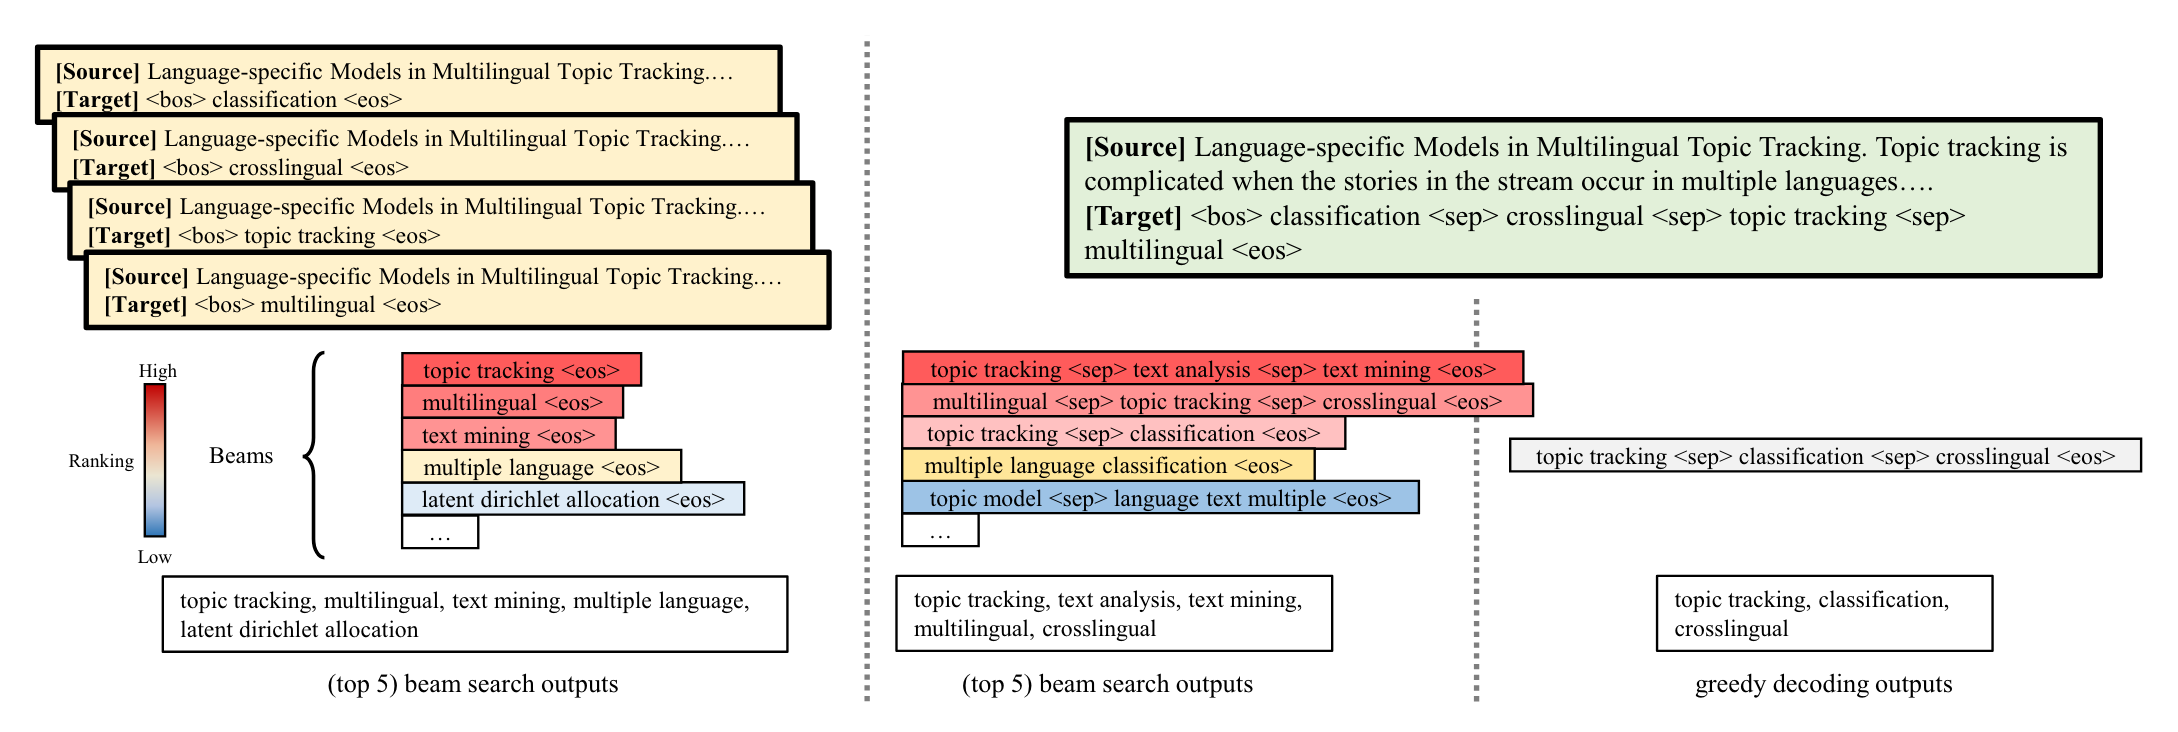
\includegraphics[width=\textwidth]{figures/o2o_o2m.png}
%\end{figure}
\end{frame}

\begin{frame}{Méthodes génératives}

    \begin{block}{CopyRNN~\cite{meng_deep_2017}}
    \begin{itemize}
        \item encodeur et décodeur récurrent bidirectionnel
        \item entraînement \textbf{one2one}
        \item mécanisme d'attention
        \item mécanisme de copie
    \end{itemize}
    \end{block}

    \only<1>{
    \begin{block}{CorrRNN~\cite{chen_keyphrase_2018}}
    \begin{itemize}
        \item entraînement \textbf{one2many}
        \item[+] mécanisme augmentant la diversité des mots-clés générés
    \end{itemize}
    \end{block}
    }
    
    \only<2>{
    \begin{block}{Autres méthodes}
    \begin{itemize}
        \item amélioration de la \textbf{diversité} des mots-clés \cite{chen_keyphrase_2018,chan_neural_2019,yuan_one_2020,chen_exclusive_2020,zhao_incorporating_2019}
        \item amélioration de la \textbf{représentation du document} \cite{chen_title-guided_2019,chen_integrated_2019}
        %\cite{ye_semi-supervised_2018} 
    \end{itemize}
    \end{block}
    }
\end{frame}

\againframe<2>{generationmethods}